% !TEX root = MAIN.tex

\section{Applicable and reference documents}

\begin{itemize}
\item{D1 - Mutation testing survey}
\item{D2 - Study of mutation testing applicability to space software}
\end{itemize}
\clearpage

\section{Terms, definitions and abbreviated terms}

\clearpage


\chapter{Code-driven Mutation Testing}

\section{General description}
\label{codeDriven}



\subsection{Product perspective}

\RQ{} The code-driven mutation testing component (in Section~\ref{codeDriven} referred to as \emph{the system}) implements the Mutation Testing Process for code-driven mutation testing described in D2.

\clearpage
\subsection{General capabilities}

\RQ{} The code-driven mutation testing component shall implement the process for the evaluation of test suite effectiveness that is drafted in Figure~\ref{fig:process:codeDriven:evaluation}. Figure~\ref{fig:process:codeDriven:evaluation} relies on UML activity diagram notation. In Figure~\ref{fig:process:codeDriven:evaluation} the execution of specific software artefacts from the end user is made explicit. Also, we use black arrows to draw control-flow, red arrows for data-flow. Each activity is described in Section~\ref{sec:rquirements:capabilities}.

\begin{figure}[h]
  \centering
	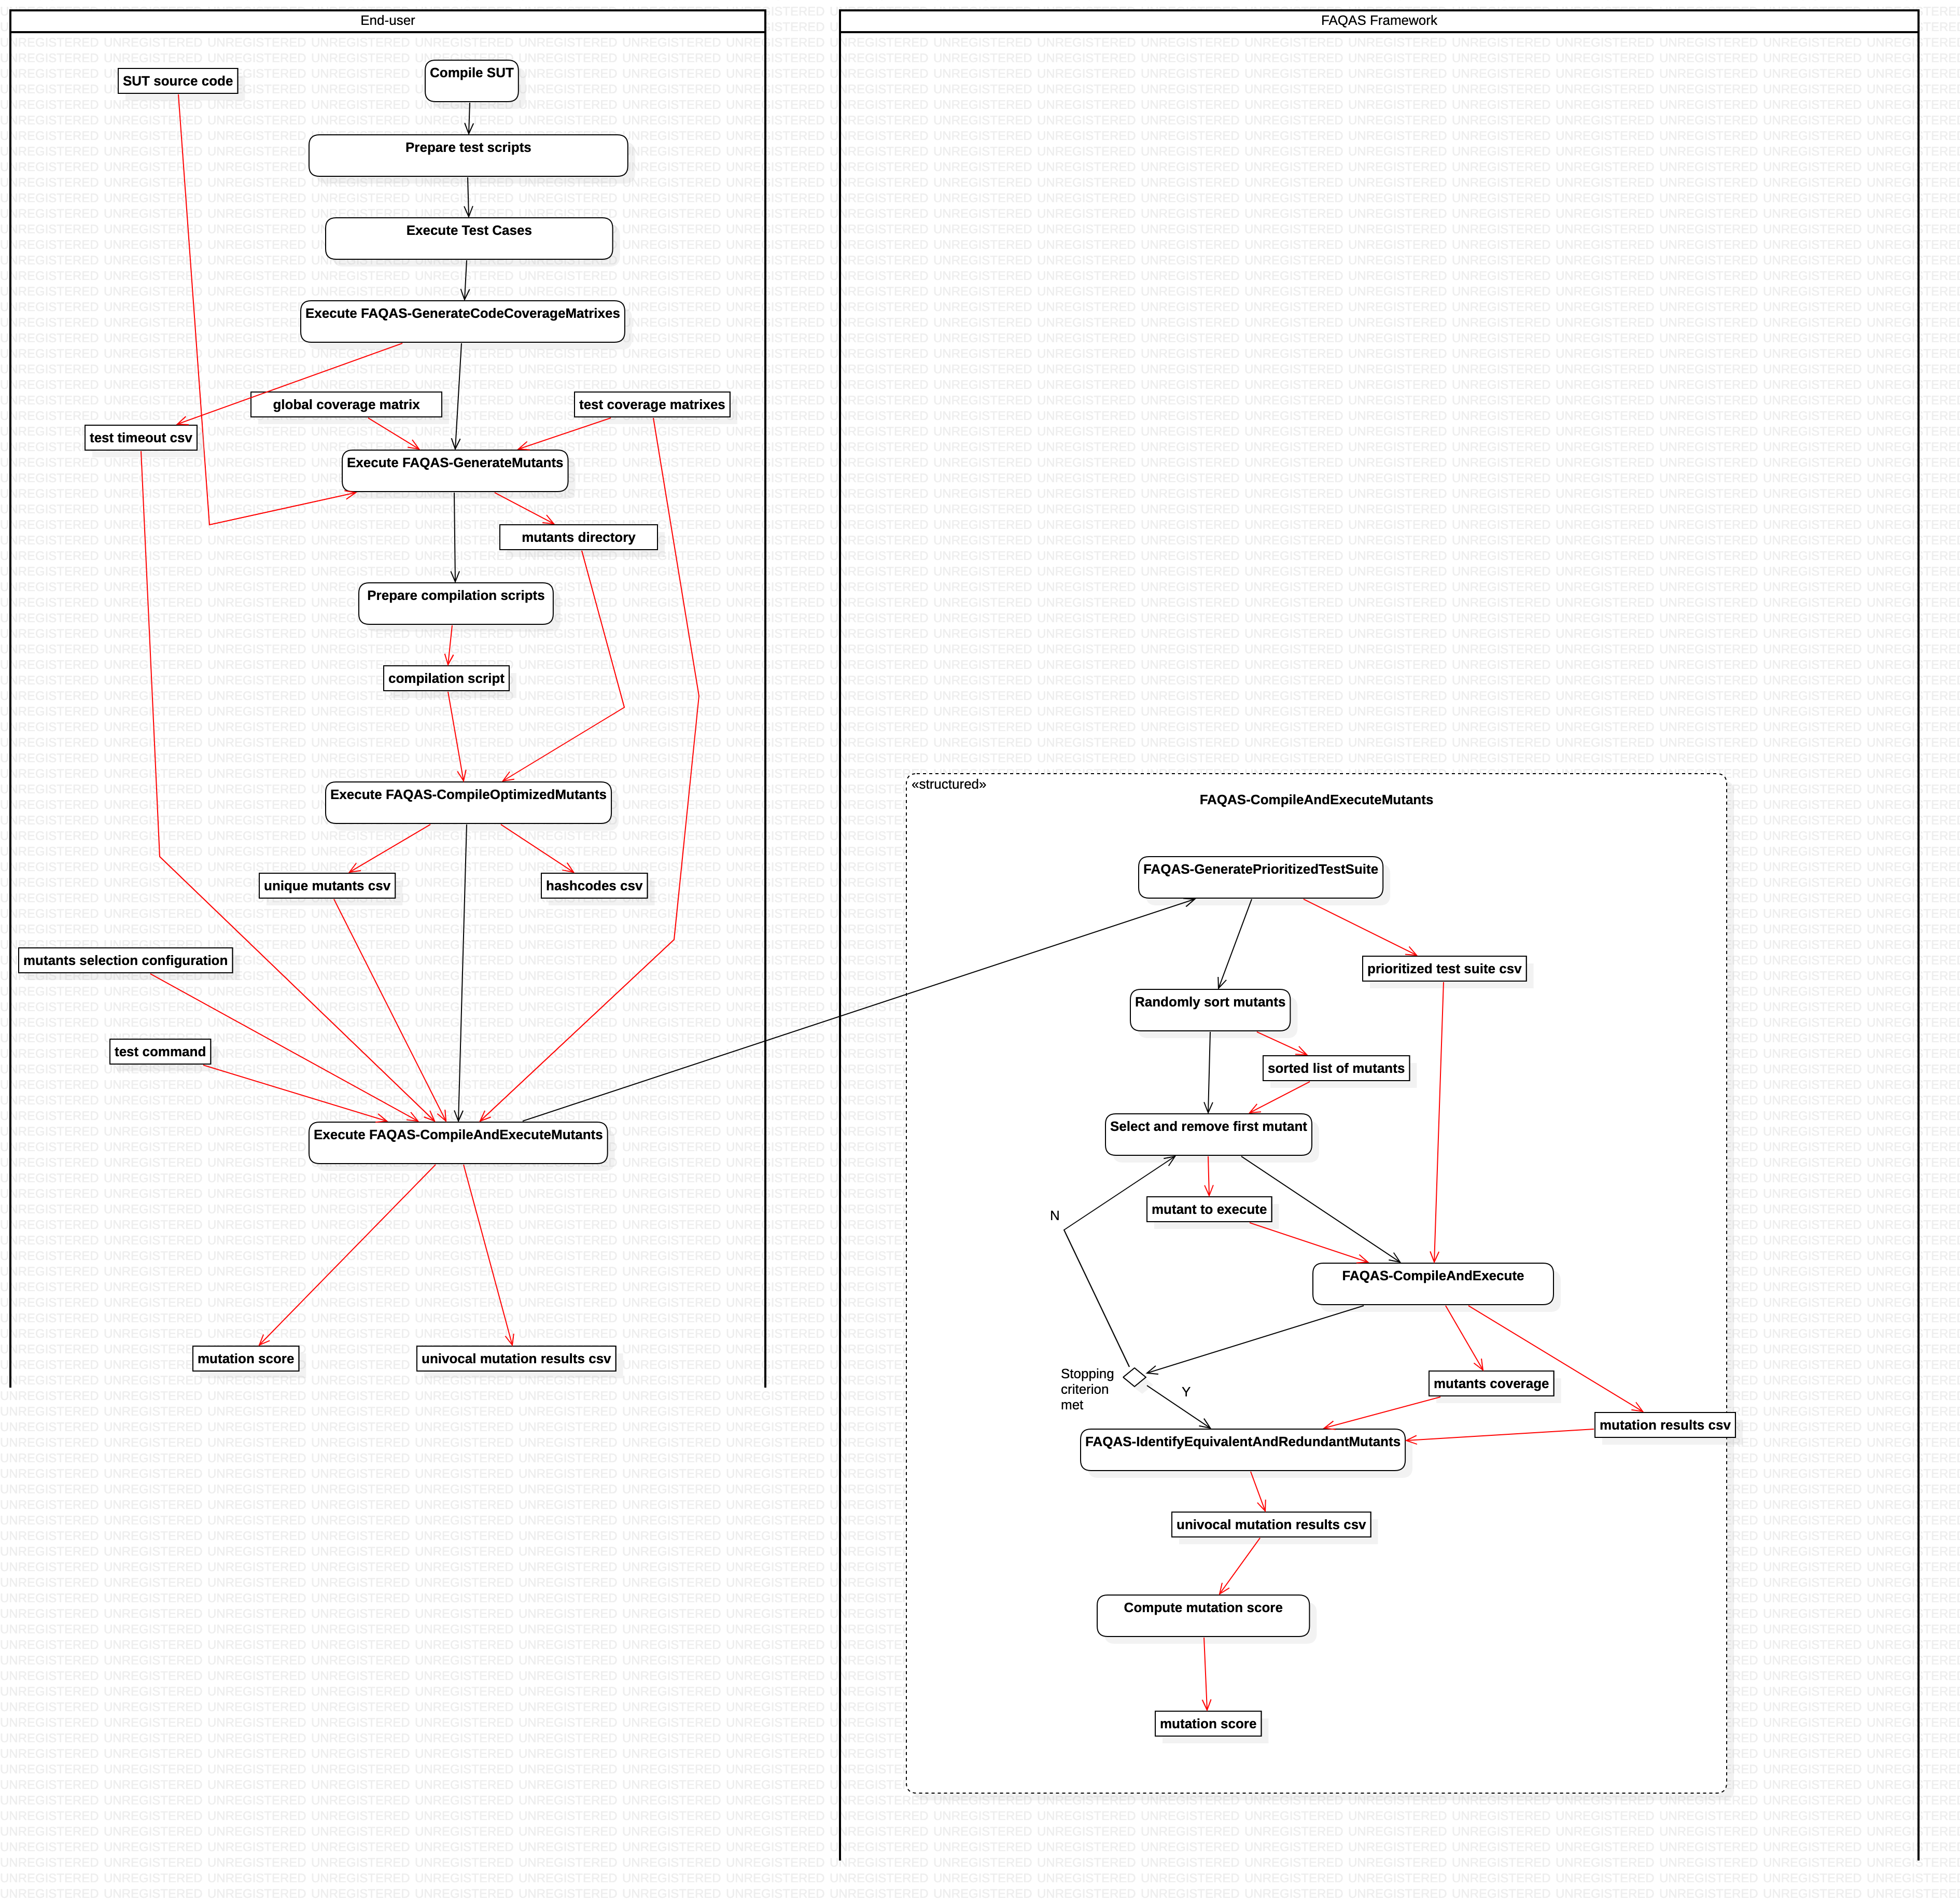
\includegraphics[width=15cm]{images/png/Activity1!CodeDrivenTestSuiteEvaluation_1.png}
      \caption{Overview of the code-driven mutation testing process to evaluate test suite effectiveness.}
      \label{fig:process:codeDriven:evaluation}
\end{figure}


\clearpage

\subsection{General constraints}


\clearpage

\subsection{Operational environment}

% cosi generale?
\RQ{} The system works with a Linux operating system and Bash shell.



\subsection{Assumptions and dependencies}

\RQ{} The system targets SUT built using either GCC Make~\footnote{https://gcc.gnu.org/onlinedocs/gccint/Makefile.html} or WAF\footnote{https://waf.io/}.

\RQ{} The system targets SUT compiled with GCC~\footnote{https://gcc.gnu.org}.

\section{Specific requirements}
%\section{General}
\subsection{Capabilities requirements}
\label{sec:rquirements:capabilities}

\RQ{} The gcov coverage information associated to each test case shall be stored in a separate directory.

\RQ{} The activity \emph{Compile SUT} in Figure~\ref{fig:process:codeDriven:evaluation} concerns the compilation of  the SUT with coverage options enabled.

\RQ{} The activity \emph{Prepare test scripts} in Figure~\ref{fig:process:codeDriven:evaluation} concerns extending the test scripts to store the code coverage of each single test case separately. This is achieved by adding a call to a dedicated bash script provided by FAQAS (\emph{FAQAS-CollectCodeCoverage}).

\RQ{} The activity \emph{Execute test cases} in Figure~\ref{fig:process:codeDriven:evaluation} concerns the execution of the test cases following the practice for the SUT.

\RQ{} The activity \emph{Execute FAQAS-GenerateCodeCoverageMatrix} in Figure~\ref{fig:process:codeDriven:evaluation} concerns the execution of a provided python program delivered with the FAQAS framework.

\RQ{} The activity \emph{Execute FAQAS-GenerateCodeCoverageMatrix} in Figure~\ref{fig:process:codeDriven:evaluation} generates a set of files: 
\begin{itemize}
\item one csv file referred to as \emph{global coverage matrix}, which indicates, for every line of code of the SUT, the ID of the test cases that cover the line of code;
\item a number of files  referred to as \emph{test coverage matrix}, one for each test case of the SUT. Each file indicates, for every line of code of the SUT, the number of times it has been covered during a single execution of the test case;
\item one file with the timeout after which we can consider a test case as non terminated (used in later stages). It is obtained by multiplying the test execution time times three.
\end{itemize}



\RQ{} Activity \emph{Execute FAQAS-GenerateMutants} in Figure~\ref{fig:process:codeDriven:evaluation} concerns the execution of the program \emph{FAQAS-GenerateMutants}. 

\RQ{} \emph{FAQAS-GenerateMutants} automatically generates a number of copies of each source file. Each copy contains one mutant.

% per ora abbiamo solo testato SRCIRor con files .c, dobbiamo valutare se funziona correttamente anche per .cpp
\RQ{} \emph{FAQAS-GenerateMutants} mutates source files with extension .c and .cpp.

\RQ{} \emph{FAQAS-GenerateMutants} generates mutants by applying a set of mutation operators that can be selected by the end-users.

\RQ{} \emph{FAQAS-GenerateMutants} implements the set of operators listed in Table~\ref{table:operators}

% !TEX root =  ../Main.tex

\newcommand{\op}{\mathit{op}}
\newcommand{\ArithmeticSet}{ \texttt{+}, \texttt{-}, \texttt{*}, \texttt{/}, \texttt{\%} }
\newcommand{\LogicalSet}{ \texttt{&&}, \texttt{||} }
\newcommand{\RelationalSet}{ \texttt{>}, \texttt{>=}, \texttt{<}, \texttt{<=}, \texttt{==}, \texttt{!=} }
\newcommand{\BitWiseSet}{ \texttt{\&}, \texttt{|}, \land }
\newcommand{\ShiftSet}{ \texttt{>>}, \texttt{<<} }


\begin{table}[h]
\caption{Implemented set of mutation operators.}
\label{table:operators} 
\centering
\scriptsize
\begin{tabular}{|@{}p{4mm}@{}|@{}p{2cm}@{\hspace{1pt}}|@{}p{11.1cm}@{}|}
\hline
&\textbf{Operator} & \textbf{Description$^{*}$} \\
\hline
\multirow{7}{*}{\rotatebox{90}{\emph{Sufficient Set}}}&ABS               & $\{(v, -v)\}$	\\
\cline{2-3}
&AOR               & $\{(\op_1, op_2) \,|\, \op_1, \op_2 \in \{ \ArithmeticSet \} \land \op_1 \neq \op_2 \} $       \\
&    			  & $\{(\op_1, \op_2) \,|\, \op_1, \op_2 \in \{\texttt{+=}, \texttt{-=}, \texttt{*=}, \texttt{/=}, \texttt{\%} \texttt{=}\} \land \op_1 \neq \op_2 \} $       \\
\cline{2-3}
&ICR               & $\{i, x) \,|\, x \in \{1, -1, 0, i + 1, i - 1, -i\}\}$           \\
\cline{2-3}
&LCR               & $\{(\op_1, \op_2) \,|\, \op_1, \op_2 \in \{ \texttt{\&\&}, || \} \land \op_1 \neq \op_2 \}$            \\
&				  & $\{(\op_1, \op_2) \,|\, \op_1, \op_2 \in \{ \texttt{\&=}, \texttt{|=}, \texttt{\&=}\} \land \op_1 \neq \op_2 \}$            \\
&				  & $\{(\op_1, \op_2) \,|\, \op_1, \op_2 \in \{ \texttt{\&}, \texttt{|}, \texttt{\&\&}\} \land \op_1 \neq \op_2 \}$            \\
\cline{2-3}
&ROR               & $\{(\op_1, \op_2) \,|\, \op_1, \op_2 \in \{ \RelationalSet \}\}$            \\
&				  & $\{ (e, !(e)) \,|\, e \in \{\texttt{if(e)}, \texttt{while(e)}\} \}$ \\
\cline{2-3}
&SDL               & $\{(s, \texttt{remove}(s))\}$            \\
\cline{2-3}
&UOI               & $\{ (v, \texttt{--}v), (v, v\texttt{--}), (v, \texttt{++}v), (v, v\texttt{++}) \}$            \\   
\hline
\hline
\multirow{5}{*}{\rotatebox{90}{\emph{OODL}}}&AOD               & $\{((t_1\,op\,t_2), t_1), ((t_1\,op\,t_2), t_2) \,|\, op \in \{ \ArithmeticSet \} $       \\ 
\cline{2-3}
&LOD               & $\{((t_1\,op\,t_2), t_1), ((t_1\,op\,t_2), t_2) \,|\, op \in \{  \} \}$       \\ 
\cline{2-3}
&ROD               & $\{((t_1\,op\,t_2), t_1), ((t_1\,op\,t_2), t_2) \,|\, op \in \{ \RelationalSet \} \}$       \\ 
\cline{2-3}
&BOD               & $\{((t_1\,op\,t_2), t_1), ((t_1\,op\,t_2), t_2) \,|\, op \in \{ \BitWiseSet \} \}$       \\ 
\cline{2-3}
&SOD               & $\{((t_1\,op\,t_2), t_1), ((t_1\,op\,t_2), t_2) \,|\, op \in \{ \ShiftSet \} \}$       \\ 
%\hline
%COR               & $\{(\op_1, \op_2) \,|\, \op_1, \op_2 \in \{ \texttt{\&\&}, \texttt{||}, \land \} \land \op_1 \neq \op_2 \}$            \\
\hline
\hline
\multirow{3}{*}{\rotatebox{90}{\emph{Other}}}&LVR			& $\{(l_1, l_2) \,|\, (l_1, l_2) \in \{(0,-1), (l_1,-l_1), (l_1, 0), (\mathit{true}, \mathit{false}), (\mathit{false}, \mathit{true})\}\}$\\
&&\\
&&\\
\hline
\end{tabular}

$^{*}$Each pair in parenthesis shows how a program element is modified by the mutation operator. Th eleft element of the pair is replaced with the right element. We follow standard syntax~\cite{kintis2018effective}. Program elements are literals ($l$), integer literals ($i$), boolean expressions ($e$), operators ($\op$), statements ($s$), variables ($v$), and terms ( $t_i$, which might be either variables or literals).
\end{table}


% quindi, non produrremo anche una lista coi nomi dei mutanti + la sua location?
\RQ{} \emph{FAQAS-GenerateMutants} generates as output a directory tree (\emph{mutants directory} in Figure~\ref{fig:process:codeDriven:evaluation}) that follows the structure of the source directory tree of the SUT. However, every source file is replaced by a folder having the same name. The folder contains all the mutants generated for that file. Every mutant has a name that univocally identify it. The mutant name results from the conjunction of the following information:
source file name, mutated function name, mutated line, mutation operator name, mutation operation, mutated “column” (i.e., char position from the beginning of the line).








\RQ{} Activity \emph{Prepare compilation scripts} in Figure~\ref{fig:process:codeDriven:evaluation} concern the modification of the main compilation script for the SUT. The engineer is expected to perform the following manual activities:
\begin{itemize}
\item Remove debugging flags
\item Remove coverage flags
\item Add placeholder for compiler optimization option
\item Add a 'sort' command in the source dependency list to ensure that source files are always compiled in the same order
\end{itemize}



\RQ{} Activity \emph{Execute FAQAS-CompileOptimizedMutants} in Figure~\ref{fig:process:codeDriven:evaluation} concerns the execution of the program \emph{FAQAS-CompileOptimizedMutants}.

\RQ{} The program \emph{FAQAS-CompileOptimizedMutants} compiles every mutant multiple times; once for every compiler optimization option selected by the end-user. It implements pseudocode in Figure~\ref{alg:CompileOptimizedMutants}.

\begin{figure}[h]
\begin{algorithmic}[1]

%\footnotesize
\scriptsize


\Require \emph{OPT}, the set of compiler optimization options specified by the end-user
\Require \emph{MutantsDir}, path to the directory tree containing the mutants
\Require \emph{SUTsources}, path of the folder containing the sources of the SUT
\Require \emph{CompilatonCommand}, the command to execute to compile the original software

\Ensure \emph{hashcodes csv}, a csv file containing for every mutant, for every option, the SHA512 hashcode of the generated executable

\Ensure \emph{unique mutants}, a csv file containing the list of unique mutants. Unique mutants are mutants that are not equivalent nor redundant. See D2 for details.
% (source inputs, follow-up inputs, output data).

\For {OPT in OPTS}
\For {Mutant in MutantsDir}
\State Compile \emph{Mutant} with program \emph{FAQAS-CompileAndExecute}
\State Generate a SHA512 hash of the generated executable
\State Put the generated SHA512 hash in the \emph{hashcodes csv} file
\EndFor
\EndFor

\State Process \emph{hashcodes csv} and identify \emph{unique mutants}
\State Save the list of \emph{unique mutants} in the output \emph{unique mutants csv} file

\end{algorithmic}
\vspace{-3mm}
\caption{FAQAS-CompileOptimizedMutants: Algorithm for compiling mutants with multiple optimization options}
%\vspace{-0.2cm}
\label{alg:CompileOptimizedMutants}
\end{figure}




\RQ{} Activity \emph{Execute FAQAS-CompileAndExecuteMutants} in Figure~\ref{fig:process:codeDriven:evaluation} concerns the execution of the program \emph{FAQAS-CompileAndExecuteMutants}.

\RQ{} The program \emph{FAQAS-CompileAndExecuteMutants} iterates over three activities (implemented by separate executable program that are inkoved automatically without user intervention): \emph{FAQAS-GeneratePrioritizedTestSuite}, \emph{FAQAS-CompileAndExecute}, \emph{FAQAS-IdentifyEquivalentAndRedundantMutants}.

\RQ{} The program \emph{FAQAS-CompileAndExecuteMutants} takes as inputs the mutants selection configuration, the unique mutants csv, the path of the SUT source folder, the command to execute test cases, and the path to the folder containing the test coverage matrixes.

\RQ{} The program \emph{FAQAS-CompileAndExecuteMutants} implements the four mutants selection strategies described in D2: \emph{all mutants}, \emph{proportional uniform sampling}, \emph{proportional method-based sampling}, \emph{uniform fixed-size sampling}, and \emph{uniform FSCI sampling}.

\RQ{} The \emph{mutants selection configuration} indicates the mutants selection strategy and a configuration value to specify the number of mutants to consider, which depends on the strategy; the value may indicate the percentage of mutants to sample (for \emph{proportional uniform sampling}, \emph{proportional method-based sampling}), the number of mutants to sample (for \emph{uniform fixed-size sampling}), the size of the confidence interval (for \emph{uniform FSCI sampling}).

\RQ{} The program\emph{FAQAS-GeneratePrioritizedTestSuite} takes as input the test coverage matrices and generate a file that specifies, for every line of the SUT, the prioritized list of test cases to execute (\emph{prioritized test suite csv}). This file indicates the sequence of test cases to execute for every mutants concerning a specific line.

\RQ{} The activity \emph{Randomly sort mutants} indicates that  \emph{FAQAS-CompileAndExecuteMutants} generate a randomly prioritized list of mutants to compile and execute from the \emph{unique mutants csv}.
In the case of \emph{proportional method-based sampling}, the list contains a set of mutants selected by following the stratified sampling strategy.

\RQ{} The activity \emph{Select and remove first mutant} indicates that  \emph{FAQAS-CompileAndExecuteMutants} select the first mutant in \emph{sorted list of mutants} and remove it from the list.

\RQ{} The program \emph{FAQAS-CompileAndExecute} compiles a mutant by running the makefile of the original program; then it executes the SUT test suite. It follows the algorithm in Figure~\ref{alg:compileAndExecute}.


\begin{figure}[h]
\begin{algorithmic}[1]
\scriptsize
\Require \emph{Mutant}, path of the mutant to compile
\Require \emph{SUTsources}, path of the folder containing the sources of the SUT
\Require \emph{CompilatonCommand}, the command to execute to compile the original software
\Require \emph{TestCommand}, the command to execute to execute a single test case
\Require \emph{TestCases}, the prioritized list of test cases for the line of the mutant
\Require \emph{TestTimeout}, the max execution time that can be taken by the test case
\Ensure \emph{Result} KILLED or LIVE, based on test execution result (i.e., all test cases pass or one test case fails)
\State put \emph{Mutant} in place of the file it has been derived (\emph{original file}), keep the original file in a safe place
\State execute  \emph{CompilatonCommand} inside \emph{SUTsources}
\For {TestCase in TestCases}
\State execute the \emph{TestCase} by running \emph{TestCommand} inside \emph{SUTsources}
% succede qualcosa strano quando scrivi "the"
\If {the \emph{TestCase} fails (i.e., \emph{TestCommand} terminates with an error code)}
\State set \emph{Result} as KILLED
\State break the for loop
\EndIf
\If {a the \emph{TestTimeout} expires}
\State set \emph{Result} as KILLED
\State break the for loop
\EndIf
\EndFor
\State move code coverage information in a subfolder of \emph{mutants coverage dir}
\State restore \emph{original file}
\end{algorithmic}
\caption{FAQAS-CompileAndExecute: Algorithm to compile and test mutants}
\label{alg:compileAndExecute}
\end{figure}

\RQ{} The program \emph{FAQAS-CompileAndExecute} collects the mutation results of every mutant in a file, \emph{mutation results csv}. It contains for every mutant the indication of the mutation result (KILLED/LIVE).

\RQ{} The program \emph{FAQAS-CompileAndExecute} compiles and execute mutants till a termination criteria is met. The termination criteria depends on the mutants selection strategy:
\begin{itemize}
\item \emph{all mutants}: the list \emph{sorted list of mutants} is empty
\item \emph{proportional uniform sampling}: a number of mutants matching the selected percentage has been executed
\item \emph{proportional method-based sampling}: the list \emph{sorted list of mutants} is empty
\item \emph{uniform fixed-size sampling}: a number of mutants matching the selected value has been executed
\item \emph{uniform FSCI sampling}: the confidence interval computed from \emph{mutation results csv} is smaller than the lenght specified by the user.
\end{itemize}

\RQ{} The program \emph{FAQAS-IdentifyEquivalentAndRedundantMutants} relies on code coverage information stored in \emph{mutants coverage dir} to identify equivalent and redundant mutants using the distance criterion $D_C$ (see D2).

\RQ{} The program \emph{FAQAS-IdentifyEquivalentAndRedundantMutants} generates a copy of \emph{mutation results csv} (i.e., \emph{univocal mutation results csv}) where only mutants that are considered non-equivalent and non-redundant are reported.

\RQ{} The activity \emph{Compile mutation score} concerns the computation of the mutation score based on the mutation results reported in \emph{univocal mutation results csv}.

\subsection{System interface requirements}

\RQ{} The main user interface for the system is the command line.

\subsection{Adaptation and missionization requirements }

None foreseen.

\subsection{Computer resource requirements}

\RQ{} The system should be executed on a Linux operating system.

\subsection{Security requirements }

\RQ{} The system should not use ports or use network connections.

\subsection{Safety requirements}

None foreseen.

\subsection{Reliability and availability requirements}

None foreseen.

\subsection{Quality requirements}

None foreseen.

\subsection{Design requirements and constraints}

\RQ{} The system should be released with ESA Software Community Licence Permissive – v2.3”, as defined at https://essr.esa.int/. Any reused component should be compatible with the licence.

\subsection{Software operations requirements}

None foreseen.

\subsection{Software maintenance requirements}

None foreseen.

\subsection{System and software observability requirements}

\RQ{} To enable post-mortem debugging, all the temporary files generated by the FAQAS executables should be kept.

\section{Verification, validation and system integration}
 \subsection{Verification and validation process requirements}
 
 \RQ{} Every mutation operator should be tested by a dedicated unit test.
 
 \RQ{} A system test suite for the whole software should be provided. It should be based on MLFS case study.
 
   \RQ{} The system should enable the computation of the mutation score for the FAQAS case study systems indicated in deliverable D2.
 
 \subsection{Validation approach}

\RQ{} SnT is expected to perform a preliminary validation of the delivered framework.

 \RQ{} FAQAS industry partners are expected to use the system at their premises to validate it.
 

%  
% \subsection{Validation requirements}
% 
%
% 
% \subsection{Verification requirements}
% 
% \RQ{}

 \section{System models}
 
 None reported.

